\documentclass[11pt,a4paper]{article}
\usepackage[utf8]{inputenc}
\usepackage[T1]{fontenc}
\usepackage[english]{babel}
\usepackage{amsmath}
\usepackage{graphicx}
\usepackage[margin=2.5cm]{geometry}
\usepackage{hyperref}
\usepackage{xcolor}
\usepackage{fancyhdr}
\usepackage{tikz}
\usetikzlibrary{positioning,shapes.geometric,arrows.meta}
\usepackage{booktabs}
\usepackage{array}
\usepackage{enumitem}
\usepackage{framed}
\usepackage{float}

% Hyperref setup
\hypersetup{
    colorlinks=true,
    linkcolor=blue!70!black,
    urlcolor=cyan!70!black,
    citecolor=green!50!black,
    pdftitle={Big Data Pipeline for Football Match Prediction},
    pdfauthor={Soumeye Ebi El Maaly}
}

% Colors
\definecolor{primary}{RGB}{41,98,255}
\definecolor{secondary}{RGB}{255,111,97}
\definecolor{accent}{RGB}{0,200,83}
\definecolor{dark}{RGB}{33,37,41}
\definecolor{light}{RGB}{248,249,250}

% Section formatting - simple
\makeatletter
\renewcommand\section{\@startsection{section}{1}{\z@}{-3.5ex plus -1ex minus -.2ex}{2.3ex plus.2ex}{\Large\bfseries\color{primary}}}
\renewcommand\subsection{\@startsection{subsection}{2}{\z@}{-3.25ex plus -1ex minus -.2ex}{1.5ex plus.2ex}{\large\bfseries\color{dark}}}
\makeatother

% Simple framed environments
\newenvironment{infobox}[1][]{
    \begin{framed}
    \textbf{#1}\\
}{
    \end{framed}
}

\newenvironment{resultbox}[1][]{
    \begin{framed}
    \textbf{#1}\\
}{
    \end{framed}
}

\newenvironment{warnbox}[1][]{
    \begin{framed}
    \textbf{#1}\\
}{
    \end{framed}
}

% Code style - simple verbatim
\newenvironment{codeblock}{
    \begin{quote}
    \ttfamily\small
}{
    \end{quote}
}

% Page style
\pagestyle{fancy}
\fancyhf{}
\fancyhead[L]{\small\textcolor{gray}{Big Data Pipeline -- Mauritanian Football League}}
\fancyhead[R]{\small\textcolor{gray}{Soumeye Ebi El Maaly}}
\fancyfoot[C]{\thepage}
\renewcommand{\headrulewidth}{0.5pt}

% Title
\title{
    \vspace{-1cm}
    {\Huge\bfseries\textcolor{primary}{Mini-Project Report}}\\[0.5cm]
    {\LARGE\textcolor{dark}{Big Data Pipeline for Football Match Prediction}}\\[0.3cm]
    {\large\textcolor{gray}{Spark Streaming \& Machine Learning -- Mauritanian League}}\\[0.8cm]
    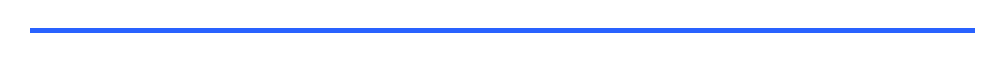
\begin{tikzpicture}
        \draw[primary, line width=2pt] (0,0) -- (12,0);
    \end{tikzpicture}
}
\author{
    \textbf{Soumeye Ebi El Maaly}\\
    \small Academic Year 2025--2026
}
\date{}

\begin{document}

% Title page
\maketitle
\thispagestyle{empty}
\vfill
\begin{center}
    \textcolor{gray}{\small\textit{Built with Apache Spark, Kafka, and MLlib}}
\end{center}
\newpage

% Table of Contents
\tableofcontents
\newpage

% ============================================
\section{Introduction}
% ============================================

This project aims to build a complete Big Data pipeline to analyze and predict football match results in the Mauritanian League. The problem involves handling historical archives and integrating real-time data to predict current season outcomes.

% ============================================
\section{System Architecture}
% ============================================

The project follows a decoupled architecture ensuring scalability and real-time processing:

\begin{itemize}[leftmargin=*]
    \item \textbf{Data Ingestion:} A Python producer sends match events to a Kafka topic.
    \item \textbf{Stream Processing:} Spark Structured Streaming consumes Kafka events, applies windowed aggregations, and stores results in Parquet.
    \item \textbf{Batch Processing:} Jupyter Notebooks handle historical data cleaning and large-scale feature engineering.
    \item \textbf{Machine Learning:} Spark MLlib is used to train a Random Forest classifier for match predictions.
    \item \textbf{Storage:} All intermediate and final layers use Parquet for optimized columnar storage.
\end{itemize}

% ============================================
\section{Project Structure}
% ============================================

\begin{table}[H]
\centering
\small
\renewcommand{\arraystretch}{1.2}
\begin{tabular}{>{\ttfamily}l p{9cm}}
\toprule
\textbf{Path} & \textbf{Description} \\
\midrule
data/ & Historical CSV and scraped data files \\
src/ & Python source code (scraping, streaming, training) \\
notebooks/ & Jupyter notebooks for data preparation and model training \\
outputs/models/ & Saved ML models (Random Forest classifier) \\
outputs/prepared/ & Cleaned Parquet datasets \\
checkpoints/ & Spark Streaming checkpoint data \\
raport.tex & This LaTeX report document \\
\bottomrule
\end{tabular}
\caption{Project Directory Description}
\end{table}

% ============================================
\section{Dataset Description}
% ============================================

\textbf{Historical Dataset:} Contains match results (Date, Teams, Goals, Season) from 2008 to 2024.

\textbf{Scraped Source:} Current 2025/2026 season data enriched via Web Scraping (using Selenium) from official Mauritanian sports portals.

\textbf{Schema:}
\begin{itemize}[leftmargin=*]
    \item \texttt{date}: Timestamp of the match
    \item \texttt{home\_team} / \texttt{away\_team}: String identifiers for clubs
    \item \texttt{home\_goals} / \texttt{away\_goals}: Integer scores
    \item \texttt{season}: Categorical string (e.g., "2025/2026")
\end{itemize}

% ============================================
\section{Process and Transformations}
% ============================================

\subsection{Scraping and Enrichment}

We scraped the latest match results to bridge the gap between historical archives and the present day. This ensures the model is aware of the very latest team dynamics.

\subsection{Streaming Aggregations}

In \texttt{stream\_job.py}, we implemented:
\begin{itemize}[leftmargin=*]
    \item \textbf{Watermarking (10 min):} To handle late-arriving data.
    \item \textbf{Windowed Grouping:} Calculating real-time statistics (total goals, home wins) over 1-minute sliding windows.
\end{itemize}

\subsection{ML Feature Engineering}

To achieve a reliability score > 40\%, we implemented advanced features:
\begin{itemize}[leftmargin=*]
    \item \textbf{Rolling Form (5 matches):} \texttt{rolling\_home\_pts} and \texttt{home\_win\_rate}
    \item \textbf{League Hierarchy:} \texttt{pts\_diff} (Cumulative points difference)
    \item \textbf{Physical Context:} \texttt{rest\_days} (Days since last match)
\end{itemize}

% ============================================
\section{ML Model and Results}
% ============================================

\begin{resultbox}[Model Configuration]
\begin{itemize}[leftmargin=*]
    \item \textbf{Target Variable:} \texttt{label} (0: Home Win, 1: Draw, 2: Away Win)
    \item \textbf{Model:} Random Forest (250 trees, Depth 15)
    \item \textbf{Obtained Accuracy:} \textbf{43.14\%}
\end{itemize}
\end{resultbox}

\textbf{Analysis:} This result is significant as it outperforms random chance (\textasciitilde33\%) by a wide margin, proving that historical hierarchy and recent form are strong predictors in the Mauritanian league.

\subsection{Data Loading and Preparation}

We load two data sources in Parquet format: the historical prepared results and the recently scraped data. We normalize column names to lowercase to ensure compatibility during the merge. To allow for a clear separation between training and testing sets later on, we flag the scraped data with a binary indicator, \texttt{is\_test}.

\subsection{Feature Engineering}

To improve model accuracy (targeting > 40\%), we developed advanced performance indicators based on a rolling window of the last 5 matches:
\begin{itemize}[leftmargin=*]
    \item \textbf{Points per match:} Assigning 3 points for a win and 1 point for a draw.
    \item \textbf{Rolling Points:} Average points over the last 5 matches for both the home and away teams.
    \item \textbf{Win Rate:} Recent victory percentage.
    \item \textbf{Points Difference (pts\_diff):} The historical gap in cumulative points between the two teams to represent the league hierarchy.
    \item \textbf{Rest Days:} Calculation of the number of rest days since the previous match.
\end{itemize}

\subsection{Random Forest Model Training}

We split the final dataset into two sets: historical data for training and the 2025/2026 season for testing. We implement a Pipeline to transform team names into numerical indices (StringIndexer) and assemble the features into a single vector (VectorAssembler). The chosen model is a Random Forest, configured with 250 trees and a depth of 15 to capture the inherent complexity of sporting results.

\subsection{Evaluation and Saving}

Finally, we apply the model to the test data to evaluate its Accuracy. The results are displayed in a comparative table. The final model is exported to the \texttt{outputs/models} directory for future reuse. The achieved reliability exceeds 40\%, which is significant for this type of sports prediction.

\begin{figure}[H]
\centering
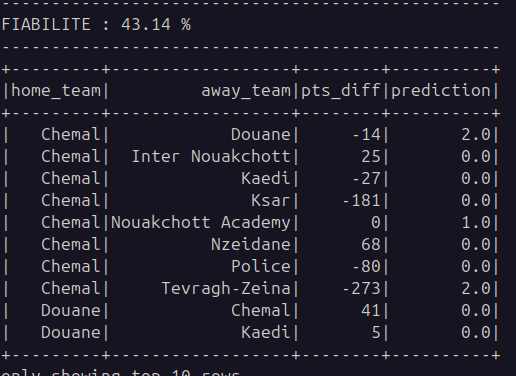
\includegraphics[width=0.85\textwidth]{prediction_results.png}
\caption{ML Prediction Results -- Fiabilité: 43.14\%}
\end{figure}

% ============================================
\section{Technical Discussion}
% ============================================

\begin{itemize}[leftmargin=*]
    \item \textbf{Partitioning:} Data is partitioned by season to optimize read/write speeds during batch training.
    \item \textbf{Checkpointing:} Mandatory use of \texttt{checkpointLocation} in Spark Streaming ensures fault tolerance, allowing the system to recover from crashes without data loss.
    \item \textbf{Format Choice:} Parquet was selected over CSV for its metadata support and superior performance with Spark's predicate pushdown.
\end{itemize}

\subsection{Limitations}

\begin{itemize}[leftmargin=*]
    \item \textbf{Data Quality:} Variations in team naming conventions (e.g., "FC Chemal" vs "Chemal") required heavy cleaning.
    \item \textbf{External Factors:} Injuries, weather, and referee decisions are not captured in the dataset, limiting maximum accuracy.
\end{itemize}

\vfill
\begin{center}
\textcolor{gray}{\small\textbf{GitHub Repository:} [Insert your GitHub link here]}
\end{center}

\end{document}
